% !TEX root = lab2_.tex
\begin{enumerate}
	\item Go to \href{https://www.overleaf.com/register}{\tt https://www.overleaf.com/register}
	\item Register for a free account (probably best to use your university email.)  You'll have to create a password at this point---make a note of it.\footnote{Overleaf isn't exactly a ``high stakes'' setting, your password needn't be super complicated---just don't re-use a password that protects a more critical account!}
	\item It's probably best to skip their ``Try the premium version for free'' offer.
    \item Click the ``Create First Project'' button---choose a blank project and name it ``hello.''
    \item You'll see two main panels (there's also some junk above and to the left, but ignore all that for now.)  The left-hand panel contains the \LaTeX\ source code for your project and the right-hand panel gives a preview of the resulting document.
    \item The ``blank project'' isn't completely blank.  The source code panel will be pre-populated with:
\medskip

\begin{codeblock}
\begin{verbatim}
 \documentclass{article}
 \usepackage{graphicx} % Required for inserting images

 \title{hello}
 \author{myemail}
 \date{August 2023}

 \begin{document}

 \maketitle

 \section{Introduction}

 \end{document}
\end{verbatim}
\end{codeblock}

\clearpage

You should see your document on the right side. It has a title section (which is 
what the \verb+\maketitle+ command created) and a section heading (this is what the \verb+\section{Introduction}+ command did). Scroll down to the bottom of the page and you
will see the number 1, the page number. Pages of articles are normally
numbered, so \LaTeX\  puts that in for you!  The area
between the \verb+\documentclass{article}+ and
the \verb+\begin{document}+ tags is known
as the \textbf{preamble} of the \LaTeX\  document. 
You should see that the preamble contains some commands that effect how the title looks.  
The default stuff that Overleaf stuck in there probably isn't quite what you want.

Let's fix that!


\item Make whatever changes you deem appropriate to the title, author and date commands. (BTW, ``date'' doesn't necessarily have to literally be the date.)  To see what the effect of your changes is, you'll need to press the ``Recompile'' button.

\item Put some words, introducing yourself after the \verb+\section{Introduction}+ command, and recompile. (There is an old and slightly unfunny tradition that the first program you write when learning a new programming language is called ``hello world!''  Please make your introduction something other than that.)
\newcounter{interitemtemp} 
\setcounter{interitemtemp}{\value{enumi}}
\end{enumerate}

At this point the source code might look something like:
\bigskip

\begin{codeblock}
\begin{verbatim}
\documentclass{article}
\usepackage{graphicx} % Required for inserting images

\title{My first LaTeX document}
\author{Ima Dumi}
\date{just checking that I can put whatever I want in the date}

\begin{document}

\maketitle

\section{Introduction}

Something other than that.

\end{document}
\end{verbatim}
\end{codeblock}

\clearpage

Which should render like so:


\begin{center}
\fbox{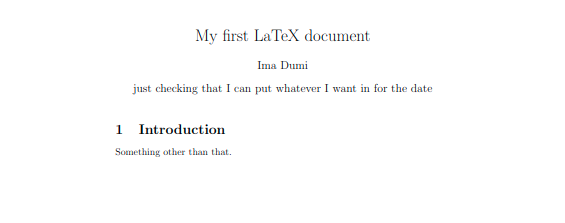
\includegraphics[width=6in]{HelloWorldScreenshot.png}}
\end{center}


\subsection*{Adding a list}

Now add a list of your three favorite classes of all time---of course
math class is first on your list, so that one has been put in for
you. You'll have to supply the next two...

\begin{enumerate}
\setcounter{enumi}{\value{interitemtemp}}

\item Copy and paste the following markup into your document 
after your greeting, but before \verb+\end{document}+.
\bigskip

\begin{codeblock}
\begin{verbatim}
\par
My three favorite classes of all time are

\begin{enumerate}
  \item Math
\end{enumerate}
\end{verbatim}
\end{codeblock}
\bigskip

Notice that the \verb+\par+ tag does not have a begin
or end. It only marks where a new paragraph should start. Same with
the \verb+\item+ tag. It only marks where a new item
in the list should start.
\item Add two items to the enumeration (and you can change the first item
if by some strange chance math is not your all time favorite class).
\item There are several list-making environments in \LaTeX.  Try some googling (Maybe ``list making latex environments'') 
and you should discover the other list-making environments.
\item Make versions of your list of favorite classes that are (1) bulleted rather than numbered, (2) name the class, and also (3) give a comment about \sout{why math is so awesome} why you liked it.
\setcounter{interitemtemp}{\value{enumi}}
\end{enumerate}

\subsection*{Adding an equation}

Equations in \LaTeX\ come in two varieties---inline and display.
An inline equation is any mathematical expression that appears in
the middle of a sentence (like the $\pi$ right here and earlier in
this document). A display equation is any mathematical expression
that should appear centered on its own line (because it's super important
or just because it's too big to put in the middle of a sentence).

To put an equation in the middle of a sentence, enclose the math between
two dollar signs (\$). To add a display equation, enclose the math
between double dollar signs (\$\$). Try it!

\begin{enumerate}
\setcounter{enumi}{\value{interitemtemp}}
\item Copy and paste the following markup into your document.
\bigskip

\begin{codeblock}
\begin{verbatim}
My favorite mathematical constant is $\pi$, but I like $e$ too.
Did you know that $$e^{i\pi}=-1?$$ Weird...
\end{verbatim}
\end{codeblock}
\bigskip

\item Notice that exponents are typeset using the same notation as used
on a calculator! Can you add markup to your document that will produce
the following?

\begin{quote}
The Pythagorean Theorem states that if a triangle has legs of lengths
$a$ and $b$ and hypotenuse of length $c$, then
\[
a^{2}+b^{2}=c^{2}.
\]
\end{quote}

\end{enumerate}
